\graphicspath{{chapters/chapter6/}}
\chapter{Analysis}

\section{The Number of Ants}
Gjør som i forrige rapport og analyser $\frac{ants}{iterations} = constant$.

%
% end The Number of Ants


\section{Pheromone Evaporation}
%
% end Pheromone Evaporation


\section{Heuristic Value in the Deposited Pheromone Levels}
if an ant discovers a solution with half the cost in the next iteration, the deposited pheromone is two 

% 
% end Heuristic Value in the Deposited Pheromone Levels


\section{Analyzing the Convergence Rates}
\textbf{Forskjellen på konvergeringen til MMAS og T-ACO} Parameterene til disse algoritmene ble optimalisert til å finne så god som mulig løsning etter 600 iterasjoner. Derfor er det ikke rettferdig å si at en algoritme er bedre enn en annen i intervallet 0 til 600 iterations. Likevel, dersom T-ACO hadde blitt terminert før 600 iterations ville den ha yielded en bedre løsning.

%
% end Analyzing the Convergence Rates


\section{How to Recognize Stagnation}
Analysere stagnation på to nivå. 1 Se på antallet nye løsninger. 2 Se på differansen mellom løsningene man genererer og det globale optima (fitness og euclidian).

%
% end How to Recognize Stagnation


\section{Comparison of Stagnation Avoidance}
MMAS proved to be less proned to stagnation than $AS_{rank}$, at the cost of having a slower convergence. The mathematics behind the pheromone limitation in MMAS implies that the lower bound $\tau_{min}$ on the pheromone strength is directly proportional to the upper bound $\tau_{max}$. The ratio between $\tau_{min}$ and $\tau_{max}$ governs the stagnation avoidance. In order to prevent stagnation the ratio must not be to great, else the edges with $\tau_{min}$ pheromone would be impossible to randomly select. On the other hand, if the ratio is too small the search would stagnate. 

Se om vi finner noen grafer som kan sammenligne hvordan T-ACO og SR-ACO klarer å unngå stagnation, imens MMAS blir stuck. Referer til tung statistikk. Hvordan stagnerer SR og FT ACO? Kan vi si noe om hvilken som er bedre i det generelle tilfellet? Når er en bedre enn den andre?

\begin{figure}[htp] % (here, top of the page, the next page)
\graphicspath{{chapters/chapter5/images/graphs/}}
%\centering
% CCNFP10g5a CCNFP12g6b CCNFP17g1b CCNFP17g1a CCNFP25g1b CCNFP25g3a CCNFP25g2a CCNFP25g7b

\begin{subfigure}[t]{0.5\textwidth}
  \centering
  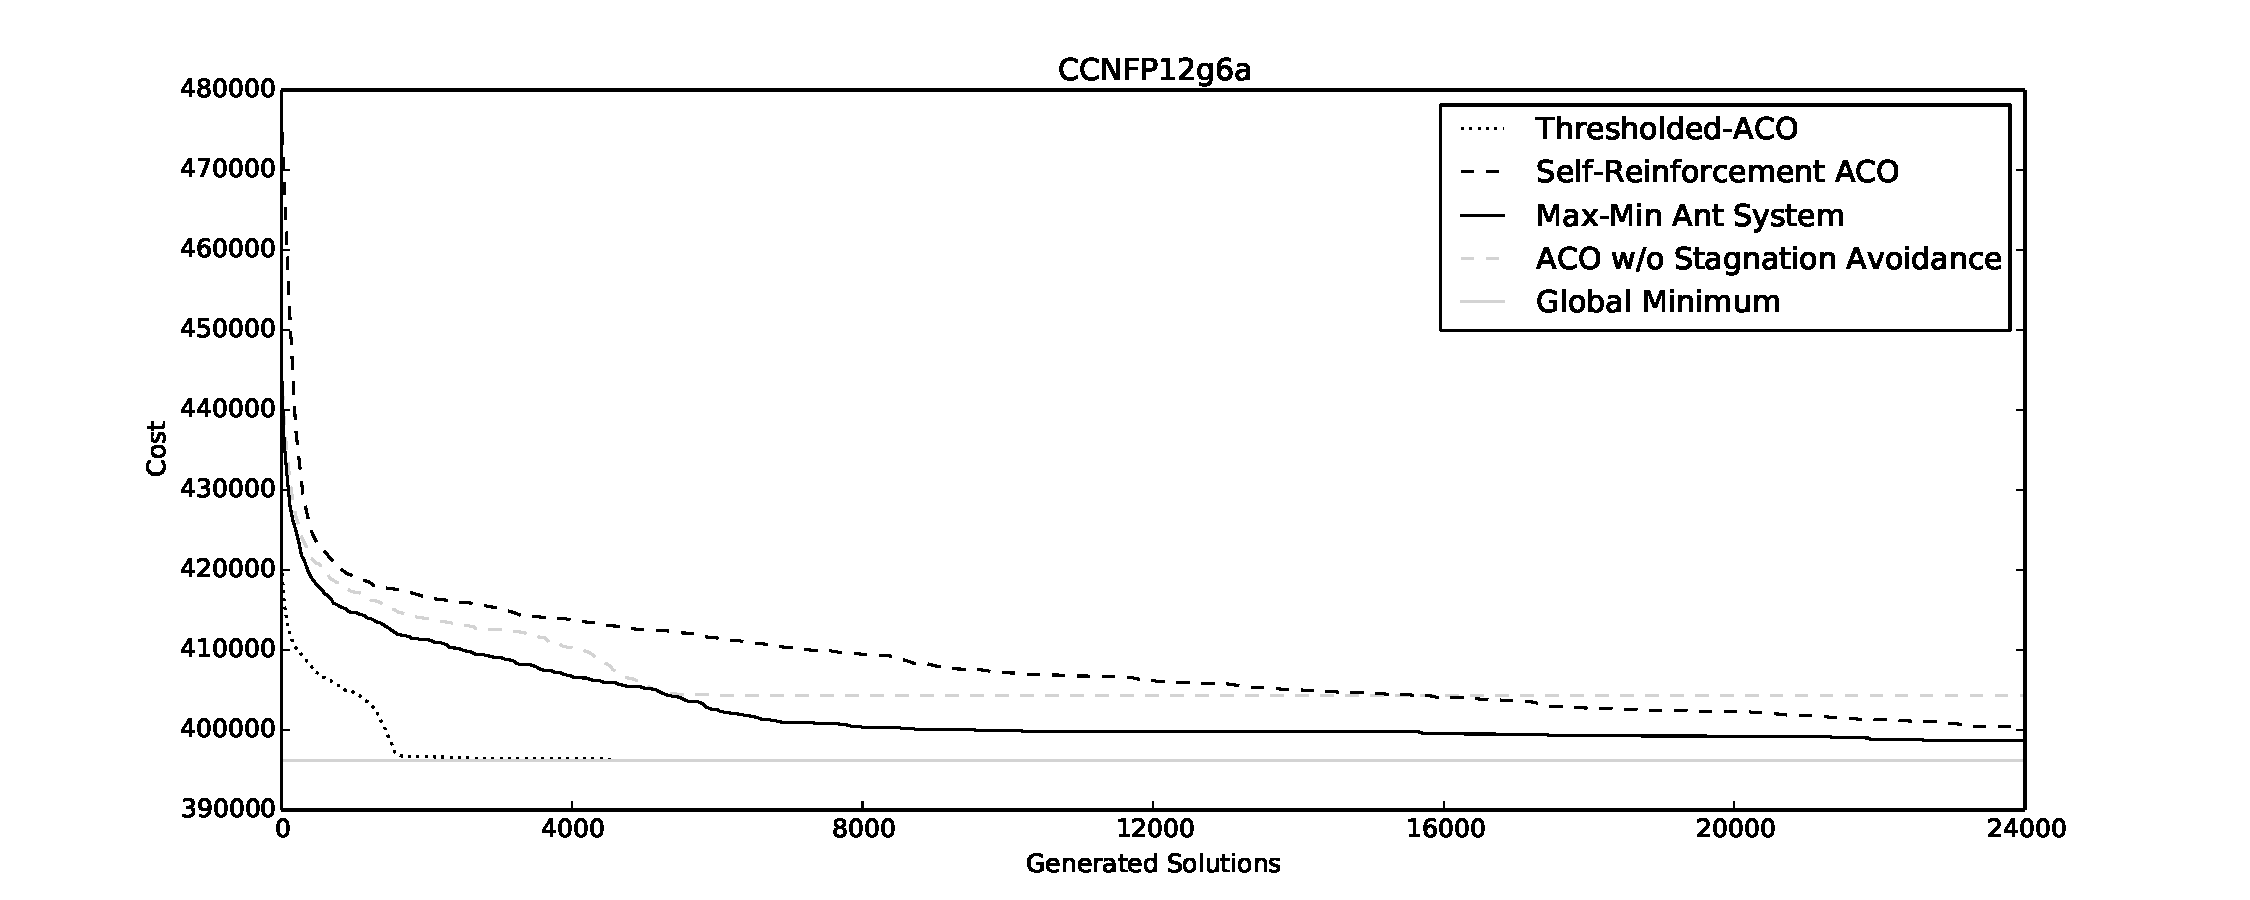
\includegraphics[width=\linewidth,height=\linewidth, keepaspectratio]{CCNFP12g6a.pdf}
  \caption{Graph CCNFP12g6a: Tresholded-ACO is the only algorithm that implements a sufficient stagnation avoidance behavior and reaches the global optima.}\label{fig:stagnation_avoidance_effeciency_fig1}
\end{subfigure}
\quad
\begin{subfigure}[t]{0.5\textwidth}
  \centering
  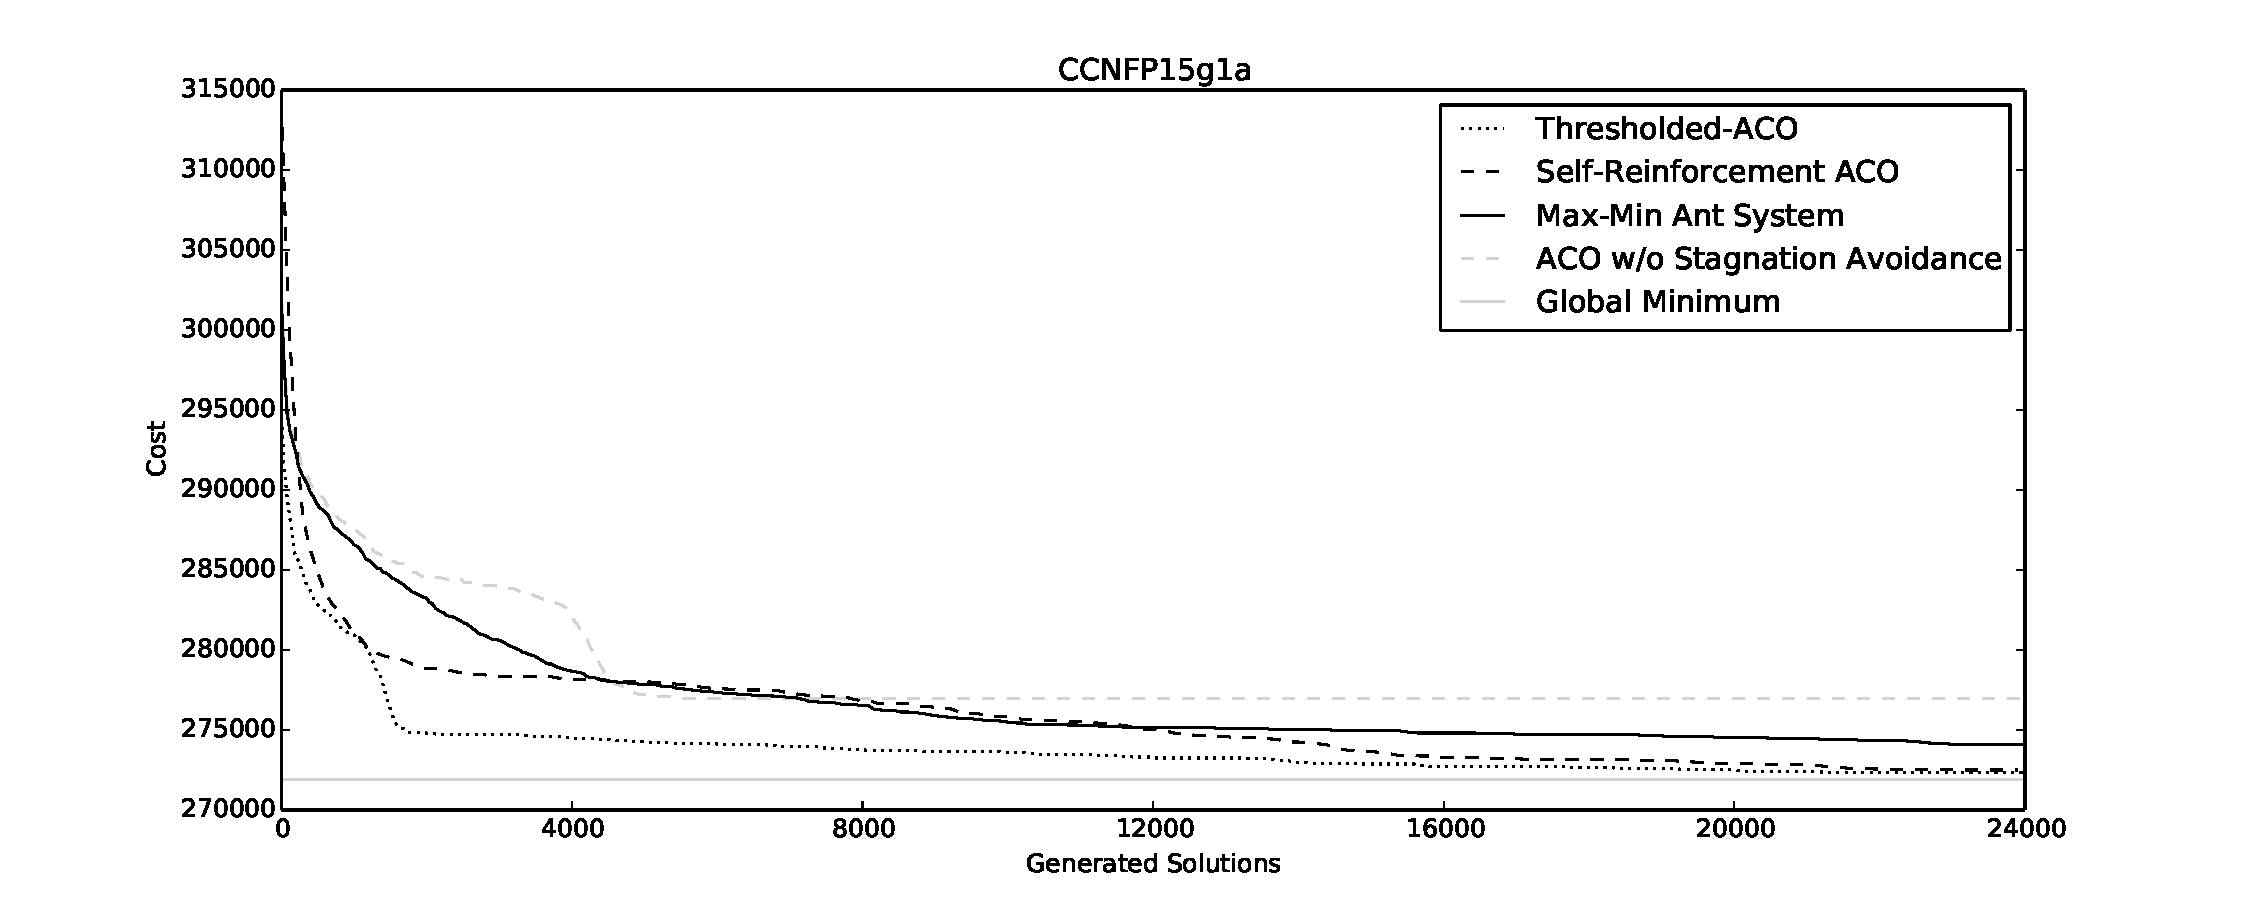
\includegraphics[width=\linewidth,height=\linewidth, keepaspectratio]{CCNFP15g1a.pdf}
  \caption{Graph CCNFP15g1a: The curves indicate slow convergence. However, the algorithms all show the ability to avoid stagnation compared to the basic algorithm. }\label{fig:stagnation_avoidance_effeciency_fig2}
\end{subfigure}

\begin{subfigure}[t]{0.5\textwidth}
  \centering
  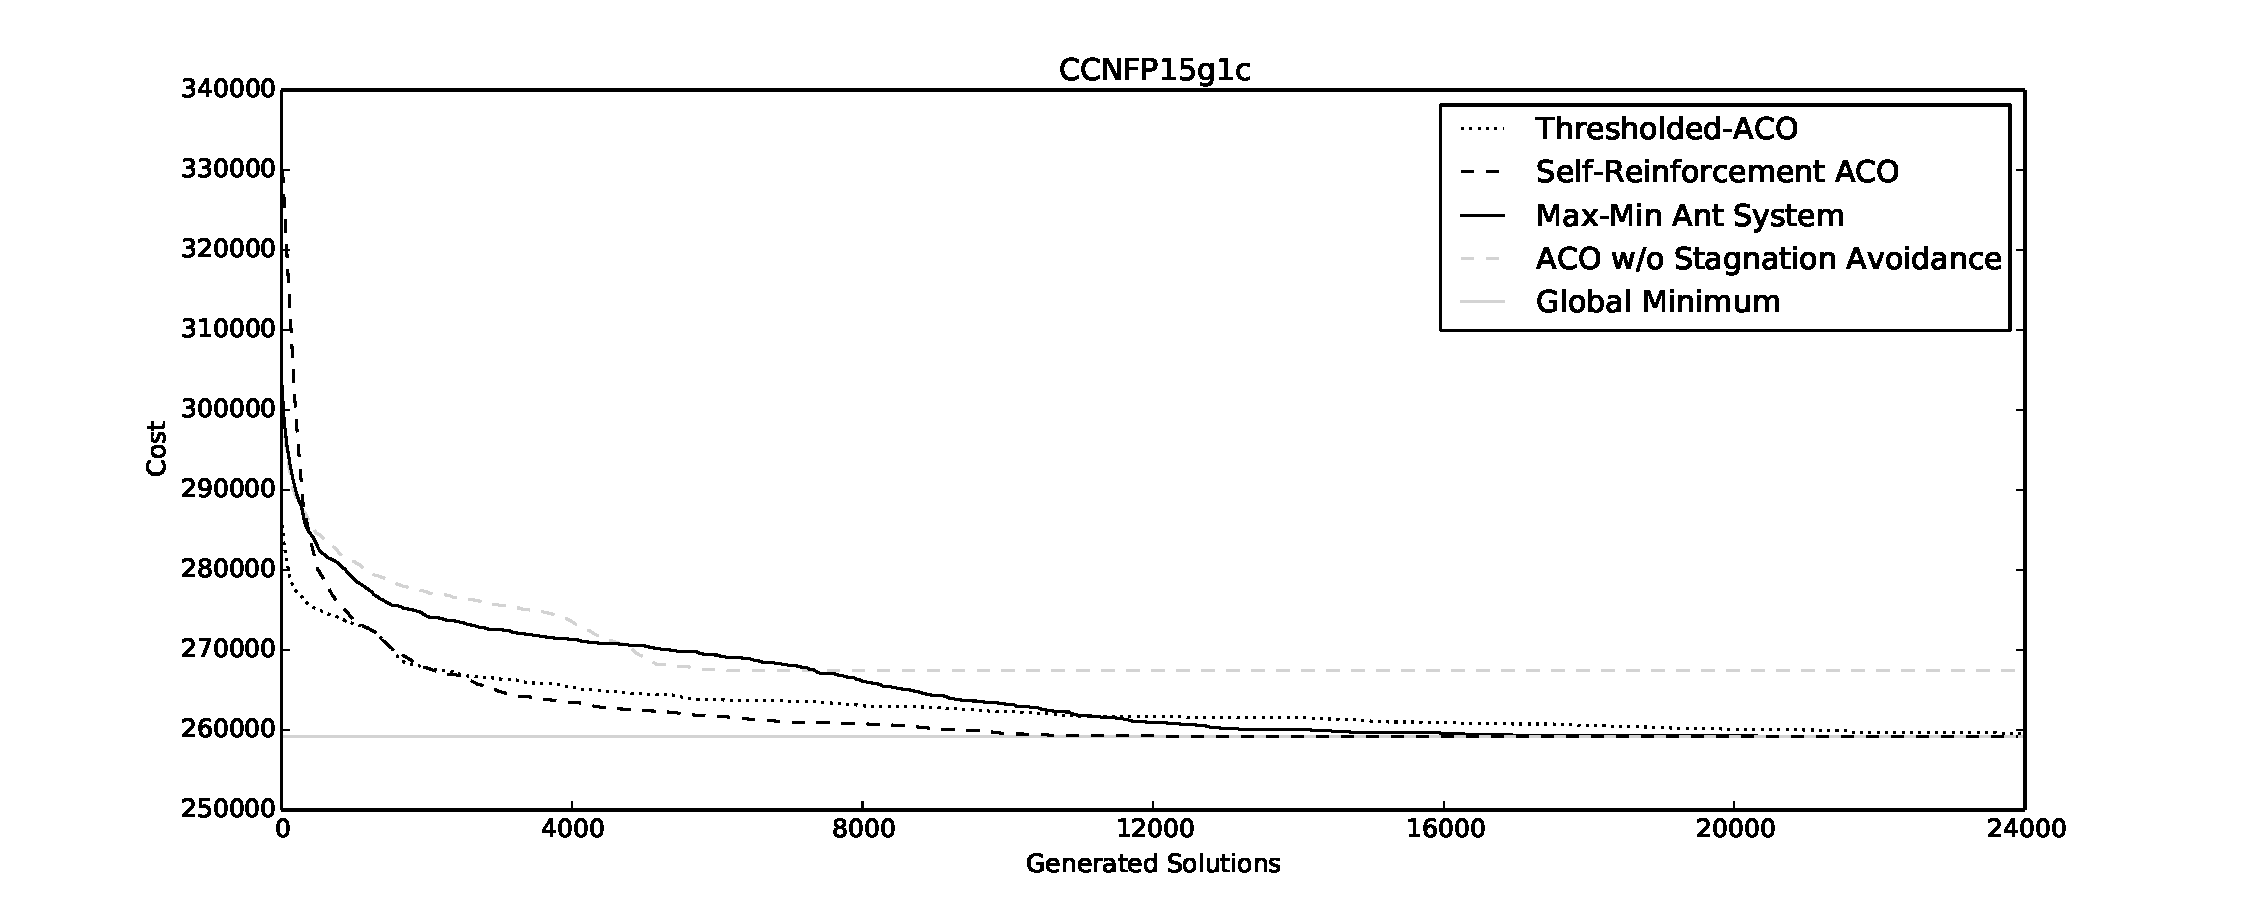
\includegraphics[width=\linewidth,height=\linewidth, keepaspectratio]{CCNFP15g1c.pdf}
  \caption{Graph CCNFP15g1c: The basic algorithm quickly stagnates to a local minimum, in contrast to the stagnation avoidance schemes that continues to converge toward the global minima. Self-Reinforcement ACO outshine the rest, while Thresholded-ACO does not reach the global optima.}\label{fig:stagnation_avoidance_effeciency_fig3}
\end{subfigure}
\quad
\begin{subfigure}[t]{0.5\textwidth}
  \centering
  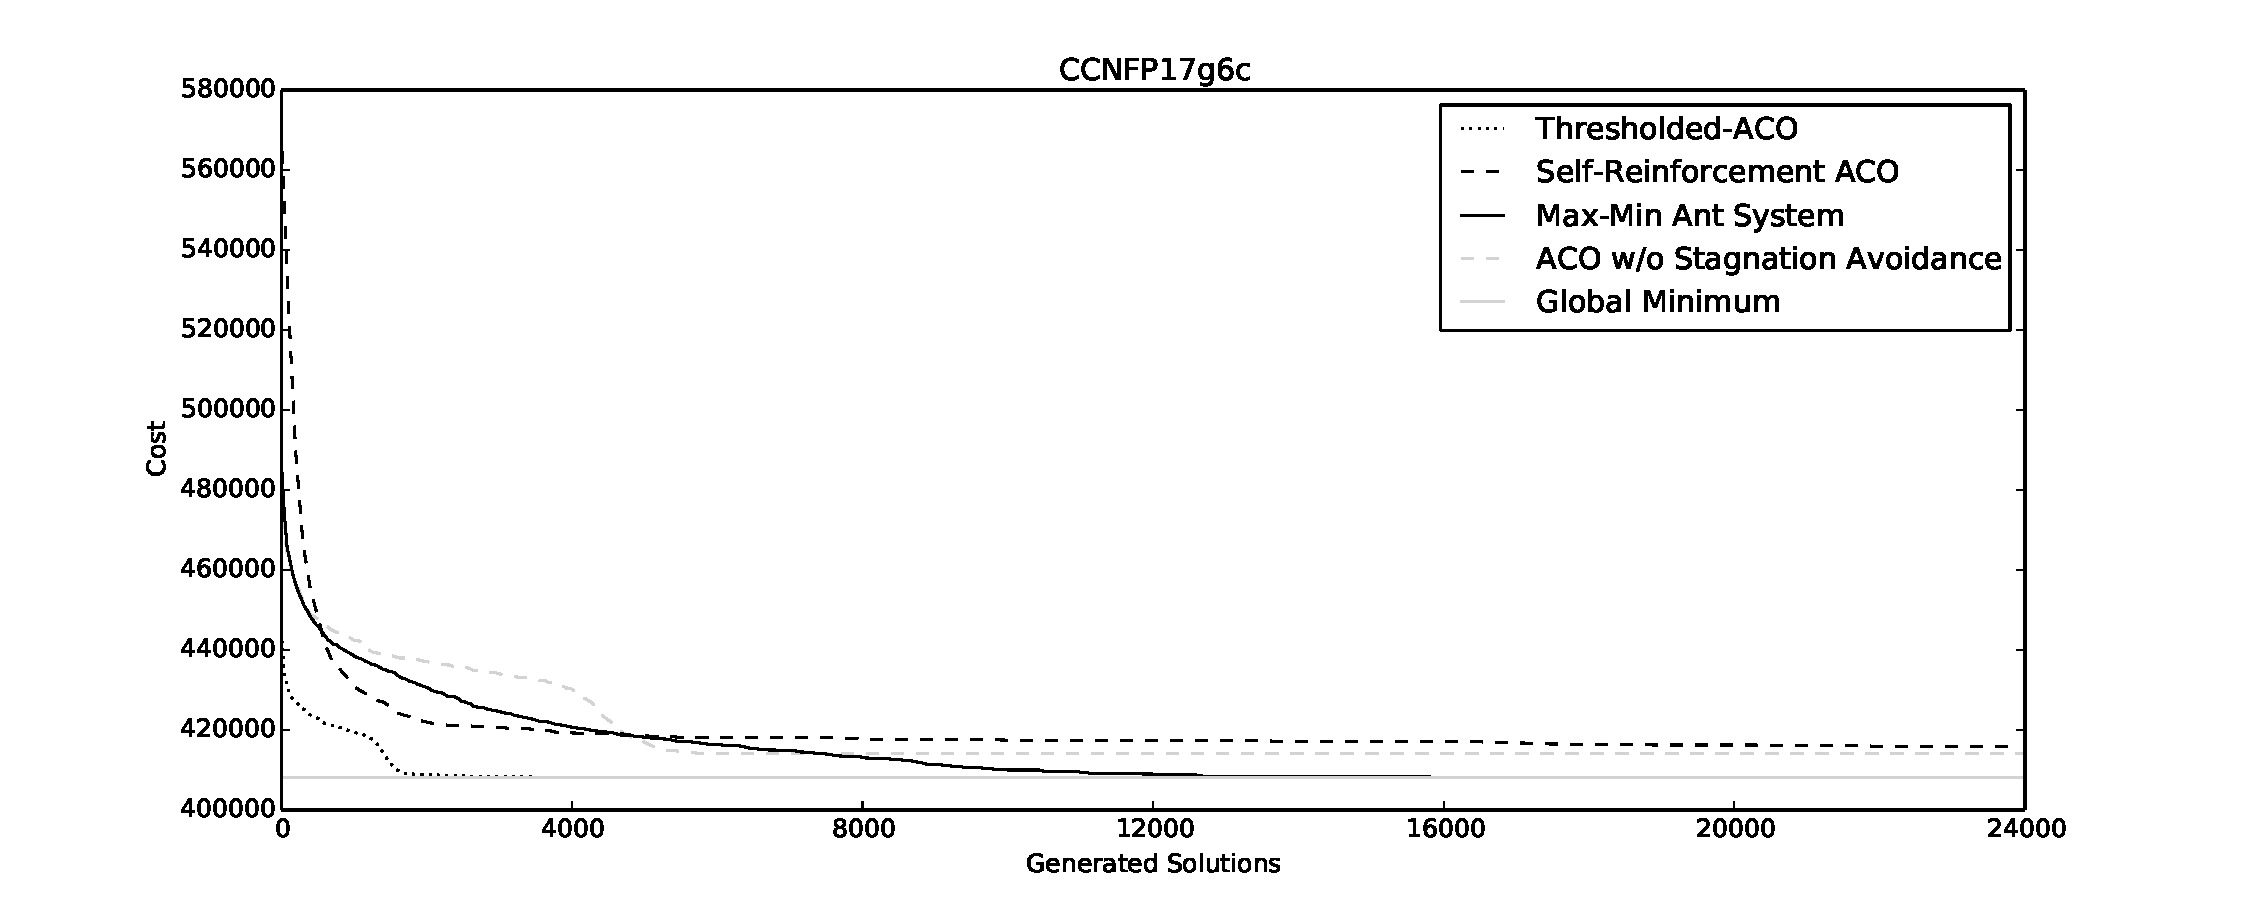
\includegraphics[width=\linewidth,height=\linewidth, keepaspectratio]{CCNFP17g6c.pdf}
  \caption{Graph CCNFP17g6c: The figure illustrates that Self-Reinforcement ACO stagnates before reaching the solution quality obtained by the basic algorithm. However, Thresholded-ACO clearly outclass the rest.}\label{fig:stagnation_avoidance_effeciency_fig4}
\end{subfigure}


\caption{Comparison of how the different stagnation avoidance schemes perform when the basic Ant Colony Optimization algorithm stagnates.}\label{fig:stagnation_avoidance_effeciency}
\end{figure}
\begin{sidewaystable}[p]
   \tiny
   \caption[Stagnation avoidance efficiency]{A comparison of how well the stagnation avoidance strategies coped with MCFP instances where the basic ACO algorithm stagnated. The table decipt the average cost of solutions from 100 runs with optimal parameter configuration. The algorithms was allowed to generate at most $24000$ solutions. The columns show the average cost, the standard deviation with respect to the discovered solution cost, and the number of solutions that was generated before reaching the global optimum. A `$-$' in the \emph{Sol} column indicate that the algorithm did not always converge to the global optimum.}
   \centering
   
   \begin{tabular}{lrrrrrrrrrrrr}
   \toprule
   
  \textbf{Graph} & \multicolumn{3}{c}{\textbf{FT\@{-}ACO}} & \multicolumn{3}{c}{\textbf{SR\@{-}ACO}} & \multicolumn{3}{c}{\textbf{MMAS}} & \multicolumn{3}{c}{\textbf{$AS_{rank}$}}\\
  \cmidrule(lr){2-4}
  \cmidrule(lr){5-7}
  \cmidrule(lr){8-10}
  \cmidrule(lr){11-13}
  & \emph{Avg} & \emph{Std} & \emph{Sol} & \emph{Avg} & \emph{Std} & \emph{Sol} & \emph{Avg} & \emph{Std} & \emph{Sol} & \emph{Avg} & \emph{Std} & \emph{Sol}\\
  \cmidrule(lr){2-2}
  \cmidrule(lr){3-3}
  \cmidrule(lr){4-4}
  \cmidrule(lr){5-5}
  \cmidrule(lr){6-6}
  \cmidrule(lr){7-7}
  \cmidrule(lr){8-8}
  \cmidrule(lr){9-9}
  \cmidrule(lr){10-10}
  \cmidrule(lr){11-11}
  \cmidrule(lr){12-12}
  \cmidrule(lr){13-13}
  
CCNFP10g05a & $6560$ & $0$ & $21080$ & \bm{$6560$} & \bm{$0$} & \bm{$600$} & $6560$ & $0$ & $4040$ & $6562$ & $9.8$ & $-$\\
CCNFP12g01b & \bm{$224040$} & \bm{$0$} & \bm{$3200$} & $224040$ & $0$ & $21100$ & $224040$ & $0$ & $7240$ & $224123$ & $833.2$ & $-$\\
CCNFP12g06b & $406792$ & $0$ & $20600$ & $406917$ & $549.3$ & $-$ & \bm{$406792$} & \bm{$0$} & \bm{$14760$} & $407932$ & $1652.6$ & $-$\\[0.7ex]
CCNFP15g01c & $259563$ & $1825.7$ & $-$ & \bm{$259242$} & \bm{$0$} & \bm{$12200$} & $259242$ & $0$ & $21480$ & $267424$ & $5161.6$ & $-$\\
CCNFP17g06c & \bm{$408075$} & \bm{$0$} & \bm{$4040$} & $415953$ & $3691.3$ & $-$ & $408075$ & $0$ & $16400$ & $414031$ & $4663.6$ & $-$\\
CCNFP25g01a & \bm{$359743$} & \bm{$0$} & \bm{$5280$} & $359743$ & $0$ & $6900$ & $359743$ & $0$ & $17280$ & $360068$ & $404.5$ & $-$\\[0.7ex]
CCNFP25g02a & \bm{$53254$} & \bm{$0$} & \bm{$3160$} & $53254$ & $0$ & $15300$ & $53254$ & $0$ & $17680$ & $53363$ & $138.6$ & $-$\\
CCNFP25g02b & \bm{$74654$} & \bm{$0$} & \bm{$2240$} & $74654$ & $0$ & $8400$ & $74654$ & $0$ & $11200$ & $74657$ & $22.0$ & $-$\\
CCNFP25g03a & \bm{$25057$} & \bm{$0$} & \bm{$15120$} & $25057$ & $0$ & $16700$ & $25057$ & $7.7$ & $-$ & $25097$ & $95.6$ & $-$\\[0.7ex]
CCNFP25g04a & $14506$ & $0$ & $11360$ & \bm{$14506$} & \bm{$0$} & \bm{$3300$} & $14506$ & $0$ & $10160$ & $14506$ & $7.7$ & $-$\\
CCNFP25g04c & \bm{$15811$} & \bm{$0$} & \bm{$2560$} & $15811$ & $0$ & $15900$ & $15811$ & $0$ & $13440$ & $15812$ & $12.9$ & $-$\\
CCNFP25g06a & $564154$ & $0$ & $21600$ & $564154$ & $0$ & $18000$ & \bm{$564154$} & \bm{$0$} & \bm{$9280$} & $564176$ & $109.9$ & $-$\\[0.7ex]
CCNFP25g07a & \bm{$83961$} & \bm{$0$} & \bm{$3280$} & $83961$ & $0$ & $12500$ & $83961$ & $0$ & $12680$ & $83979$ & $102.5$ & $-$\\
CCNFP25g07b & \bm{$123045$} & \bm{$0$} & \bm{$3880$} & $123196$ & $335.4$ & $-$ & $123045$ & $0$ & $9760$ & $123223$ & $357.2$ & $-$\\
CCNFP25g07c & $107968$ & $0$ & $10240$ & $107968$ & $0$ & $12300$ & \bm{$107968$} & \bm{$0$} & \bm{$8400$} & $108003$ & $272.3$ & $-$\\[0.7ex]
CCNFP25g08c & \bm{$31854$} & \bm{$0$} & \bm{$4080$} & $31854$ & $0$ & $15100$ & $31854$ & $0$ & $16400$ & $31875$ & $29.8$ & $-$\\
CCNFP25g10c & $21222$ & $0$ & $3440$ & \bm{$21222$} & \bm{$0$} & \bm{$1900$} & $21222$ & $0$ & $13240$ & $21222$ & $0.5$ & $-$\\
CCNFP30g06a & \bm{$857529$} & \bm{$0$} & \bm{$3040$} & $864910$ & $12636.0$ & $-$ & $857529$ & $0$ & $13440$ & $859360$ & $4209.5$ & $-$\\[0.7ex]
CCNFP30g07c & \bm{$126048$} & \bm{$0$} & \bm{$8400$} & $126765$ & $1151.2$ & $-$ & $126048$ & $0$ & $10440$ & $126059$ & $46.3$ & $-$\\
CCNFP50g03a & \bm{$29743$} & \bm{$0$} & \bm{$2920$} & $29743$ & $0$ & $23400$ & $29743$ & $0$ & $15120$ & $29745$ & $10.4$ & $-$\\
  \bottomrule
  \end{tabular}
\end{sidewaystable}

%
% end Comparison of Stagnation Avoidance


\section{Observation on Solution Similarities}
\textbf{Se på "stammen" av løsningstreet} Mange av kantene i MSTene våre er felles mellom trærene. Dette er interessant å snakke litt om. Kanskje en ide for local search?

%
% end Observation on Solution Similarities


\section{Combining Good Solutions is Ineffective}
Combining good solutions is a poor heuristic for discovering new (greater) solutions.
\textbf{Combining} combining multiple solutions is a poor idea. uniforme fordelinger (samt å kombinere løsninger) er en dårlig ide

%
% end Combining Good Solutions is Ineffective


\section{Comparing Random and Small World Graphs}
\textbf{Compare Moteiro graphs vs Small World graphs} hvilke er enklest å løse? Husk å nevne størrelsesforskjell. Hvilke algoritmer er best på disse? Husk å begrunne / bevise.

%
% end Comparing Random and Small World Graphs


\section{Analyzing Problem Hardness (?)}
\textbf{binned statistics} binned statistics (sampling distribution) for å klassifisere problem hardness

%
% end Analyzing Problem Hardness